\question{}

\begin{ابجد}
\item \textbf{نادرست}: طبق ویژگی \lr{Local Markov Property}، در شبکه‌ی بیزی هر گره به شرط مشاهده شدن والدین، از تمام گره‌های \underline{غیر نواده} خود مستقل شرطی است. بنابراین ممکن است نسبت به یکی از نوادگان خود (که فرزند مستقیم آن نیست) وابسته‌ی شرطی باشد که با عبارت بیان شده در سوال در تناقض است. \\
در مثال زیر، گره $e$ فرزند مستقیم $c$ نمی‌باشد (غیرفرزند است) و تنها مسیر $cde$ بین گره‌های $c$ و $e$ وجود دارد که فعال است، پس نمی‌توان در مورد استقلال نظر قطعی داد و ممکن است $c$ و $e$ مستقل یا وابسته‌ی شرطی باشند.
\begin{figure}[H]
    \centering
    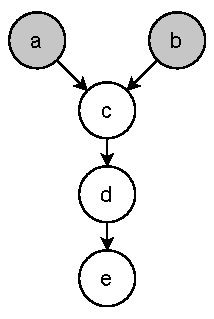
\includegraphics[width=0.2\textwidth]{assets/a1-A.pdf}
\end{figure}

\item \textbf{نادرست}: در \lr{common effect} داده شده، اگر خود $C$ یا یکی از \underline{نوادگان} آن را مشاهده کنیم مسیر بین $X$ و $Y$ فعال می‌شود.

\item \textbf{نادرست}: اگر حتی یک مسیر فعال بین $X$ و $Y$ وجود داشته باشد، این دو متغیر از هم جدا نشده‌اند و نمی‌توان به طور قطعی در مورد استقلال آنها نظر داد. (ممکن است مستقل باشند)

\item \textbf{درست}: در هر دو شبکه، به شرط مشاهده‌ی متغیر $x_2$، متغیرهای $x_1$ و $x_3$ از هم مستقل می‌شوند. محاسبه‌ی احتمال توزیع توأم در هر یک از شبکه‌ها به این صورت می‌باشد:
\begin{align}
    P_{left}(x_1, x_2, x_3) = P(x_2) \cdot P(x_1|x_2) \cdot P(x_3|x_2) \\
    P_{right}(x_1, x_2, x_3) = P(x_1) \cdot P(x_2|x_1) \cdot P(x_3|x_2)
\end{align}
طبق رابطه‌ی بیز داریم:
\begin{align*}
    P(x_1|x_2) = \frac{P(x_1) \cdot P(x_2|x_1)}{P(x_2)} \Rightarrow P(x_2) \cdot P(x_1|x_2) = P(x_1) \cdot P(x_2|x_1)
\end{align*}
بنابراین با اعمال قانون بیز، می‌بینیم که دو رابطه‌ی (1) و (2) معادل می‌شوند.

\item \textbf{درست}: در این حالت تعداد متغیرهای پنهان \footnote{hidden} مسئله $n - 2$ می‌باشد و در روش \lr{Inference by Enumeration} باید توزیع‌های توأم را به ازای تک‌تک حالت‌های متغیرهای پنهان محاسبه کنیم. همچنین باید تمام حالت‌های $X$ را هم در نظر بگیریم. بنابراین با فرض اینکه محاسبه‌ی هر احتمال توأم در $O(1)$ انجام شود، پیچیدگی زمانی مسئله $O(2^{n-1}) = O(\frac{1}{2}2^n) = O(2^n)$ می‌باشد.

\item \textbf{درست}: با این کار به یک فاکتور بزرگتر می‌رسیم که هیچ گونه اطلاعات اضافه‌تری به ما نمی‌دهد.

\item \textbf{نادرست}: برای حذف یک متغیر، ابتدا باید فاکتورهای شامل آن متغیر را \lr{join} کرده و سپس با \lr{marginalize} کردن، آن متغیر را حذف کنیم. اگرچه مرحله‌ی \lr{marginalization} فاکتور ساخته شده در مرحله‌ی قبل را کوچک‌تر می‌کند، اما اگه چند فاکتور را \lr{join} کرده باشیم ممکن است فاکتور نهایی لزوماً از فاکتورهای اولیه کوچک‌تر نباشد.

\item \textbf{درست}: در شبکه‌ی بیزی یال‌ها یک‌طرفه هستند و فرزندان روی والدین اثر نمی‌گذارند. بنابراین در محاسبه‌ی احتمال شرطی یک متغیر، می‌توان فرزندان آن که جزء شواهد نیستند را در نظر نگرفت.

\item \textbf{درست}: هر رأس حداکثر $K$ پدر و هر پدر حداکثر $D$ حالت دارد. بنابراین باید احتمال حالت‌های ممکن یک متغیر را به ازای حداکثر $D^K$ حالت ممکن والدین داشته باشیم. همچنین خود آن متغیر نیز حداکثر $D$ حالت ممکن دارد که به ازای هر حالت مشخص از والدین، به $D$ سطر برای حالت‌های ممکن نیاز داریم. پس جدول هر متغیر حداکثر $D \times D^K = D^{K+1}$ سطر دارد و باید این کار را برای تمام $N$ متغیر انجام دهیم. بنابراین $N \times D^{K+1}$ یک کران بالا برای اندازه‌ی جداول است.

\item \textbf{درست}: در روش \lr{Inference by Enumeration} ابتدا کل توزیع توأم محاسبه می‌شود، در حالی که در \lr{Variable Elimination} متغیرها در اولین فرصت ممکن \lr{marginalize} (حذف) می‌شوند که این کار محاسبات تکراری را حذف کرده و سرعت را بسیار بالاتر می‌برد.

\end{ابجد}